\documentclass[11pt, a4paper, twocolumn]{article}

\usepackage{style} 

% Information for generating title
\title{\bfseries Machine Learning: Project 1}
\author{\textbf{Olivier Stähli} \\ \href{mailto:olivier.staehli@epfl.ch}{olivier.staehli@epfl.ch}
   \and \textbf{Ivan Bioli} \\ \href{mailto:ivan.bioli@epfl.ch}{ivan.bioli@epfl.ch}
   \and \textbf{Fabio Matti} \\ \href{mailto:fabio.matti@epfl.ch}{fabio.matti@epfl.ch}}
\date{}

\begin{document}

% Escaping twocolumn-layout to generate titlelines and abstract
\twocolumn[
  \begin{@twocolumnfalse}
    \vspace{-1.5cm}
    \maketitle
    \begin{abstract}
        We implement six standard versions and one optimized version of a linear
        regressor. Subsequently, the Higgs boson data set for binary classification
        from 30 numerical features is used for testing our implementations. We
        perform various preprocessing techniques and tune the parameters of our
        regressors to maximize in first priority the F1-score and in second
        priority the accuracy of the predictions.
    \end{abstract}
    \vspace{0.75cm}
  \end{@twocolumnfalse}
]

\section{Introduction}
\label{sec:introduction}

The features in the data set record numerical measurements that coincide with the observation of either a decay signature that was caused by an event involving a Higgs boson ('s' for signal) or one that is not related to Higgs boson like decays ('b' for background) \cite{higgs2014}. Based on 250'000 samples of training data, our goal is to predict the unknown labels for the test data.

\section{Models and Methods}
\label{sec:models}

\subsection{Preprocessing}
\label{subsec:preprocessing}
In preprocessing, we visualized and analyzed the data in a first step. We made modifications to the features that have many undefined values (Figure \ref{fig:undefined_values_per_feature}), which were set to -999.
We implemented the -999 values to be set to zero, mean or median. Further, we added to the features with undefined values another feature which binary indicates if the feature is defined or not. We then split the dataset according to the values of 
After that, we standardized our data set. As a final preprocessing step, we transform our data into polynomial features.


\begin{figure}[htp]
    \centering
    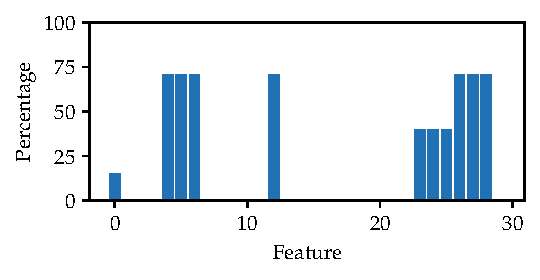
\includegraphics[width=\columnwidth]{figures/undefined_values.pdf}
    \caption{This figure displays which feature has undefined values.}
    \label{fig:undefined_values_per_feature}
\end{figure}

\subsection{Implementations}
\label{subsec:implementations}

We implemented the six proposed regressors in Python, based on their description
in \cite{jaggi2021}. Our implementations solely rely on the NumPy 1.21.1 library.
The source code is available on our Git repository\footnote{\url{https://github.com/FMatti/ML_project1}}.

We paid particular attention to the following aspects:

\begin{itemize}
    \item Robustness: We implement the regressors in such a way that they can
          be passed any NumPy ndarray object as data matrix by diligent reshaping
          of arrays. Furthermore, we included \enquote{exp-guards} that prevent exponential 
          functions from overflowing.
    \item Simple minimum working example: Each of our regressors may be fitted by 
          just passing the training data without any other parameters to the function.
    \item Thorough documentation: Every regressor's parameters and a simple usage
          example are described in a comment block below the function definition.
\end{itemize}

Since the logistic regression demonstrated in \cite{jaggi2021} only works for
$y_n \in \{0, 1\}$, we derived an equivalent formalism for the given labels
$\hat{y}_n \in \{-1, 1\}$. The derivation is found in 'addendum.pdf'
on our Git repository. The
resulting gradient of the loss function is
\begin{equation}
    \boldsymbol{\nabla} \mathcal{L}(\boldsymbol{w})
     = - \boldsymbol{X}^T \left[ \boldsymbol{y} \odot \frac{1}
        {1 + \exp{(\hat{\boldsymbol{y}} \odot (\boldsymbol{X} \boldsymbol{w}))}} \right]
\end{equation}
Here, $\odot$ denotes element-wise multiplication.

{\color{red}TODO}: Finally, we create an optimized regressor based on the following principles:

\begin{itemize}
    \item Lasso subgradient descent.
    \item ...
    \item Adjustment of label skewness: Since the training labels exhibit a skewness
          of approximately 65 to 35 \% of one category to the other, we adjust the
          classification threshold (set to zero by default) in such a way, that our
          predicted labels have the same ratio as the training labels. Otherwise,
          if for instance our prediction ratio was 50-50, and supposing the testing
          labels are of the same nature as the training labels are, we would at best
          be able to achieve an accuracy of 85 \% from the beginning.
\end{itemize}

\subsection{Parameter tuning}
\label{subsec:tuning}

{\color{red}TODO}: Explain parameter tuning (crossvalidation, grid search for ideal parameters).

\begin{figure}[htp]
    \centering
    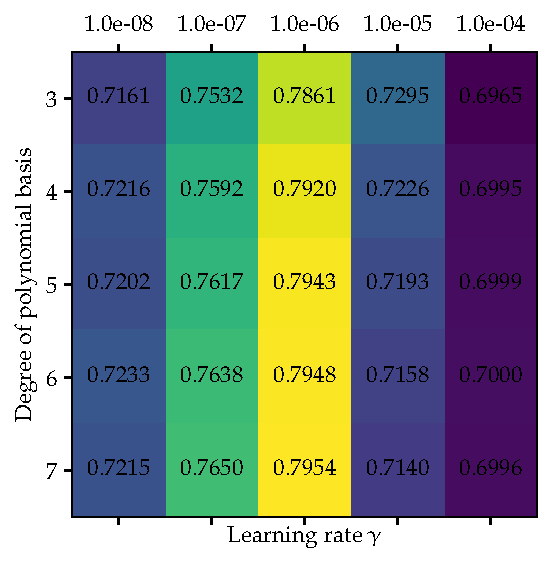
\includegraphics[width=\columnwidth]{figures/log_reg_gridsearch.pdf}
    \caption{{\color{red}TODO}: Parameter grid search 4-fold cross validation, reg logistic regression, lambda and gamma for fixed degree and max iters.}
    \label{fig:paramter_grid_search}
\end{figure}

The set of parameters that worked best for each regressor can be found in Table \ref{tab:params} below.

\begin{table}[ht]
    \caption{{\color{red}TODO}: Ideal parameters for the regressors found by means of grid-search
             and 4-fold cross-validation with the training set. $\lambda$ is 
             the regularization parameter, $N$ the maximum number of iterations,
             and $\gamma$ the learning rate. If used, the initial parameter vector
             $\boldsymbol{w}_0$ was always set to zero.}
    \label{tab:params}
    \centering
    \renewcommand{\arraystretch}{1.2}
    \begin{tabular}{@{}lccc@{}}
        \toprule
        Regressor & $\lambda$ & $N$ & $\gamma$ \\
        \midrule
        least\_squares\_GD & - & 100 & 0.1 \\
        least\_squares\_SGD & - & 100 & 0.1 \\
        least\_squares & - & - & -  \\
        ridge\_regression & 0.1 & - & - \\
        logistic\_regression & - & 100 & 0.1 \\
        reg\_logistic\_regression & 0.1 & 100 & 0.1 \\
        lasso\_SD & 0.1 & 100 & 0.1 \\
        \bottomrule
    \end{tabular}
\end{table}

\section{Results}
\label{sec:results}
The F1-score and accuracy our regressors were able to achieve can be seen below in Table
\ref{tab:results}.

% TODO: Links to submissions
\begin{table}[ht]
    \caption{Scores of the predictions we achieved with the regressors on 
             the parameters specified in \ref{tab:params}. The regressor's
             names are clickable links ({\color{red}TODO}) to the submission on AIcrowd.}
    \label{tab:results}
    \centering
    \renewcommand{\arraystretch}{1.2}
    \begin{tabular}{@{}lcc@{}}
        \toprule
        Regressor & F1-score & Accuracy \\
        \midrule
        \href{https://www.aicrowd.com/challenges/epfl-machine-learning-higgs/submissions/159686}{least\_squares\_GD} & 0.665 & 0.712 \\
        \href{https://www.aicrowd.com/challenges/epfl-machine-learning-higgs/submissions/159686}{least\_squares\_SGD} & 0.665 & 0.712 \\
        \href{https://www.aicrowd.com/challenges/epfl-machine-learning-higgs/submissions/159686}{least\_squares} & 0.665 & 0.712 \\
        \href{https://www.aicrowd.com/challenges/epfl-machine-learning-higgs/submissions/159686}{ridge\_regression} & 0.665 & 0.712 \\
        \href{https://www.aicrowd.com/challenges/epfl-machine-learning-higgs/submissions/159686}{logistic\_regression} & 0.665 & 0.712 \\
        \href{https://www.aicrowd.com/challenges/epfl-machine-learning-higgs/submissions/159686}{reg\_logistic\_regression} & 0.665 & 0.712 \\
        \href{https://www.aicrowd.com/challenges/epfl-machine-learning-higgs/submissions/159686}{optimized\_regressor} & 0.665 & 0.712 \\
        \bottomrule
    \end{tabular}
\end{table}

\section{Discussion}
\label{sec:discussion}
During implementation we learned that replacing -999 with zero, mean or median does not improve our results and that linear model is unsuited for this classification.

{\color{red}TODO}: Shortcomings of our regressors.

\bibliography{biblio.bib}

\end{document}
